\section{Database og Data Access Layer}\label{sec:designdatabase}

%\subsection{Indledende design overvejelser}
Før design af database og data access layer, er der foretaget nogle indledende tekonologiundersøgelser. DDS-lite har været brugt til at designe første udkast til databasen.

Ved videre undersøgelse af mulighederne for udvikling af database og tilhørende DAL blev Entity Framework 6.0 taget i brug. Dette er valgt da brugen af en ORM\footnote{Object Relational Mapper}, gør det lettere at integrere rå data records i et objekt orienteret system. Entity Frameworket gør det med andre ord muligt at behandle rå data records som objekter. 

Helt fra begyndelsen af databasen/DAL designfasen har tanken været at skabe et DAL der blot eksponerer et interface, der skal gøre det nemt for klienter at bruge det. Dette illustreres ved figur~\ref{fig:vs_codeMap}.

Efter Entity Framkeworket blev vedtaget til brug, blev der udarbejdet et ER diagram ved hjælp af Visual Studio's modelling project. Der er flere måder at designe databaser på i Entity Frameworket. Undervejs er flere af dem blevet afprøvet, herunder \textit{Code First}, \textit{Model First} samt \textit{Database First}.

\textit{Database first} blev brugt i forbindelse med DDS-Lite som blev brugt til at designe selve databasen. Code First tilgangen gav en bred forståelse for hvordan Entity Frameworket fungerede.

Dog blev \textit{Model First} tilgangen valgt, da der i projektets udviklingsfase ofte blev foretaget markante ændringer i designet. \textit{Model first} gør det lettere at udføre ER opdateringer, direkte på modellen og derefter køre et tilhørende SQL script direkte på databasen. Det første \textit{Model first} udkast til projektets database var meget omfattende og er sidenhen blevet revideret og omkonstrueret. Se figur~\ref{fig:databaseERD_firstattempt_uml} for dette tidlige design.

\begin{figure}[H]
	\centering
	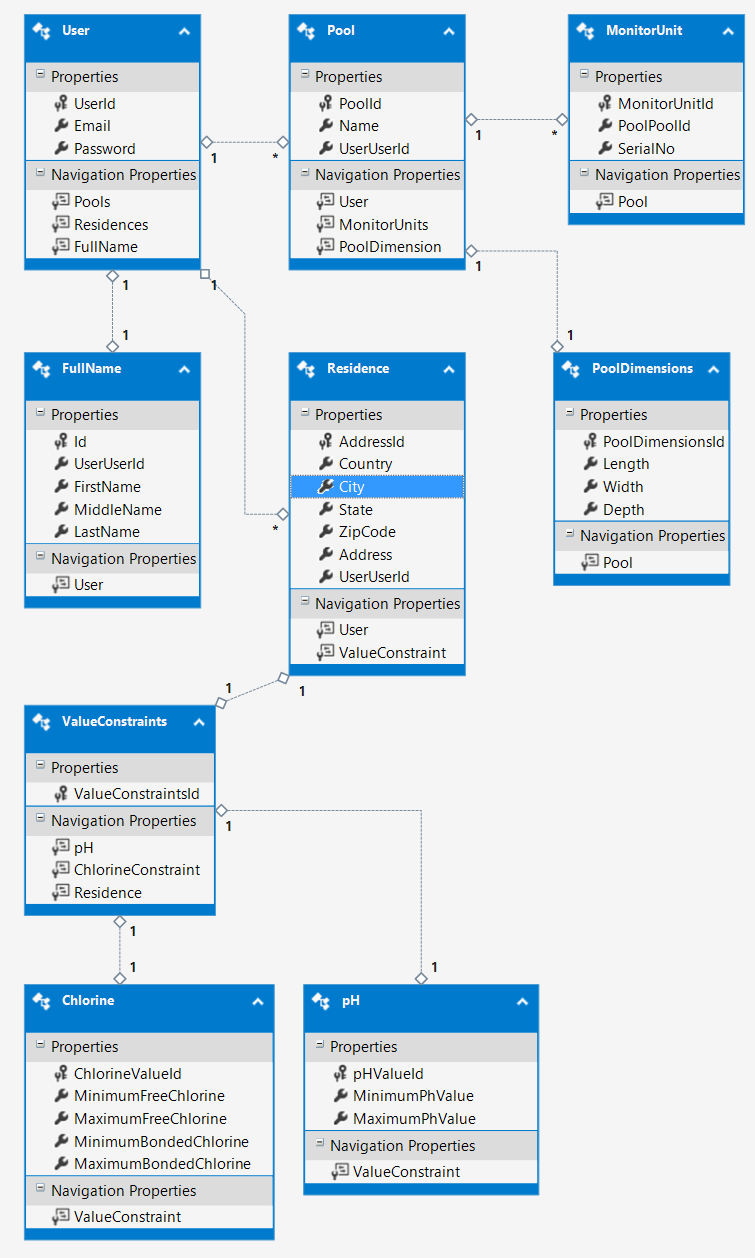
\includegraphics[width=0.8\linewidth]{figs/design/databaseERD}
	\caption{Første "Model First tilgang" til database design}
	\label{fig:databaseERD_firstattempt_uml}
\end{figure}

Af markante ændringer kan der nævnes:

\begin{itemize}
	\item FullName entiteten fjernes, User får 3 naming properties.
	\item Residence entiteten fjernes, og Pool entitens \textit{Name} property står for indhold af både addresse og navn.
	\item Value constraints fjernes helt da de ikke er nødvendige at have på databasen
	\item PoolDimensions entiteten fjernes, og Pool får en \textit{Volume} property.
	\item MonitorUnit entiteten udgår af fra databasen. Denne har kun været i databasen for at checke på et evt. serienummer.
	\item Persistering af data er blevet smartere, se figur \ref{fig:databaseERD_final_uml}.
\end{itemize}

\begin{figure}[h]
	\centering
	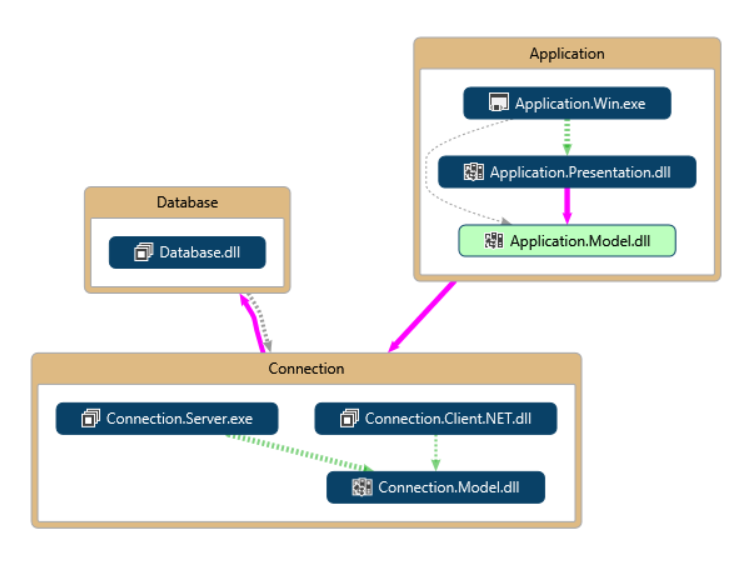
\includegraphics[width=0.8\linewidth]{figs/design/vs_codeMap.PNG}
	\caption{Dependancy graf for Smartpool Systemet}
	\label{fig:vs_codeMap}
\end{figure}

\subsection{Udvalgte User Story}

Med udgangspunkt i \gls{moscow} analysen på side~\pageref{sec:moscow} blev det første udkast til databasen lavet. Meningen var at opfylde punkterne: 

\begin{itemize}
	\item Der skal kunne oprettes en bruger til systemet.
	\item Brugeren skal kunne se sine pooldata.
\end{itemize}

For at lave dette på en måde som gjorde udvidelse let, kom første udkast til at se ud som vist på figur~\ref{fig:database_class_1}. Adgangen til databasen skulle være simpel. Dette var på grund af grænsefladen til resten af system, som skulle udvikles samtidigt. På denne måde skulle de øvrige grupper ikke ændre deres brug af \textit{ISmartpool} interfacet.  Derfor skulle der laves én klasse som ville have associationer til specialiserede klasser. Figur~\ref{fig:database_class_1} viser hvordan kaldet fra \textit{context} går gennem klassen \textit{ISmartpool}.

\begin{figure}[h]
	\centering
	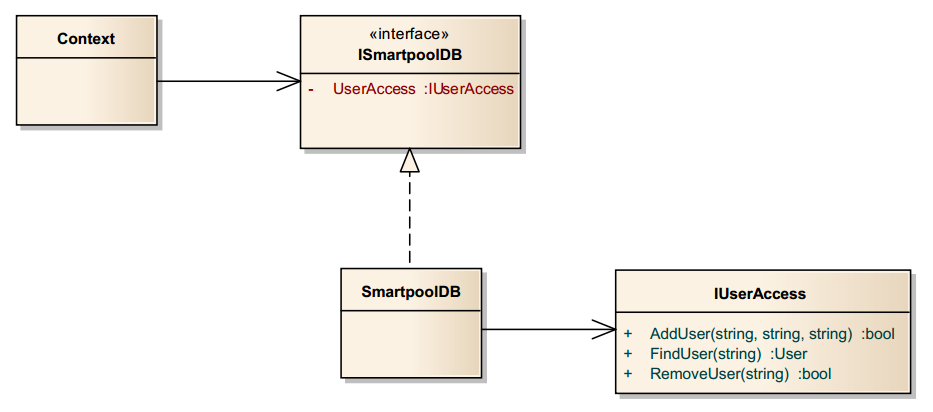
\includegraphics[width=0.9\linewidth]{figs/design/database_class_1}
	\caption{Første design for database-adgang.}
	\label{fig:database_class_1}
\end{figure}

På denne måde skulle \textit{UserAccess} klasse så stå for adgang til brugerinformationer i databasen. 

Der skulle så laves en simple database, med det eneste formål at kunne indeholde disse basale informationer om brugerne af systemet.

\begin{itemize}
	\item Navn (for, mellem og -efternavn)
	\item Email
	\item Password
\end{itemize}

Med \gls{ef} blev følgende model lavet til at opfylde dette krav.

\begin{figure}[h]
	\centering
	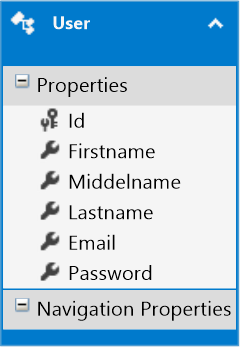
\includegraphics[width=0.25\linewidth]{figs/design/database_model_1}
	\caption{Model for første design for database-adgang.}
	\label{fig:database_model_1}
\end{figure}

Udfra dette blev et script genereret, som så skulle køres mod en localdb. Nu var databasen oprettet og implementeringen af \textit{UserAccess} klassen kunne starte.

\subsection{Persistering af sensordata}
%Husk at tage udgangspunkt historisk pool data US
Da Smartpool systemet kræver lagring af større mængder data er der gjort en del overvejelser på området. 
En tidlig udgave af database designet kan ses på figir~\ref{fig:databaseERD_final_uml}. Her gemmes alt indsamlet data i én stor tabel. Dette er uhensigtsmæssigt i forbindelse med data queries, da der på denne måde skulle søges i et meget større dataset end nødvendigt. Designet er siden blevet optimeret. 

Ser man på figur~\ref{fig:databaseERD_final_uml}, er entiteten MonitorUnit blevet fjernet. Dataen ligger her i hver sin respektive tabel med henblik på type. Der er tilføjet en Data entitet der har et timestamp som attribut. Man kan derved finde tidsspecfik data, blot ved at kende den Data entitet der kender til brugerens pool. På denne måde er søgetiden optimeret med en faktor 4. Dog vil søgetider stadig blive længere jo flere pools der tilføjes i systemet.

En videre optimering ville være at oprette nye data tabeller hver gang der oprettes en pool i systemet. Dette vil mindske søgetider drastisk. Gruppen har talt med Jesper Tørresø om dette problem, men ingen løsning blev fundet.

Envidere kan data der er ældre end x antal dage, flyttes til en anden tabel. På denne måde vil der komme et max for søgetider i nyere data.
Mulighederne for dette er undersøgt, dog vil løsningen kræve yderligere teknologiundersøgelser, samt tage for lang tid at implementere det nuværende design.

\subsubsection{User Story - Se pooldata}

"\textit{Som bruger vil jeg kunne se mine pooldata.}"\todo{Ændr denne US???}

Det endelige design tillader en bruger at hente sine egen pooldata.

Funktionaliteten hertil er implementeret i projektets data access layer. Udadtil har DAL et interface \textit{ISmartpoolDB} som en klient, \gls{windserver}, kan kalde ind i. Dette er smart da data-access klienten ikke behøves at have referencer til alle DAL klasser.

\begin{lstlisting}[caption=TokenMsgResponse constructor,label=code:tokenMsgRespone_constructor]
public TokenMsgResponse(ISmartpoolDB smartpoolDb)
{
	_smartpoolDb = smartpoolDB;
	...
}
\end{lstlisting}

Som det kan ses på kodeudsnit~\ref{code:tokenMsgRespone_constructor}, initialiseres objektet i klientens constructor.
For at få data trukket ud af databasen kaldes DAL's DataAccess klasse som implementerer DataAccess interfacet IDataAccess. DataAccess har de nødvendige data getter metoder. 
Alle getData metoder returnerer en liste af tupler. Tuplerne indeholder enum SensorTypes, som beskriver hvilken sensor der har foretaget målingen, og en double der repræsenterer målingens værdi.

\begin{lstlisting}[caption=something, label=code:derp]
private List<Tuple<SensorTypes, List<double>>> GetSensorValues(string userName, string poolName, int days)
{
	return new List<Tuple<SensorTypes, List<double>>>
		{
			GetData(_smartpoolDb.DataAccess.GetTemperatureValues(userName, poolName, days), SensorTypes.Temperature),
			GetData(_smartpoolDb.DataAccess.GetPhValues(userName, poolName, days), SensorTypes.Ph),
			GetData(_smartpoolDb.DataAccess.GetChlorineValues(userName, poolName, days), SensorTypes.Chlorine),
			GetData(_smartpoolDb.DataAccess.GetHumidityValues(userName, poolName, days), SensorTypes.Humidity)
		};
}
\end{lstlisting}\todo{missing caption!}

\begin{figure}[h]
	\centering
	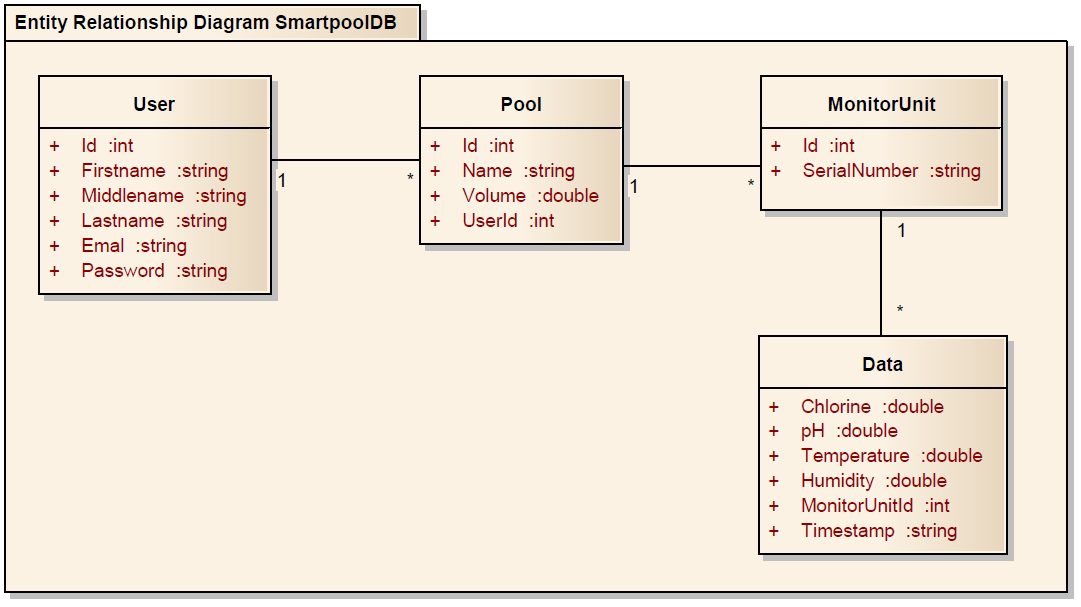
\includegraphics[width=\linewidth]{figs/design/databaseERD_old_uml}
	\caption{Første udgave af ER diagram, UML notation}
	\label{fig:databaseERD_old_uml}
\end{figure}

Sensor data persisteres i hver sin tabel.

\subsection{Endeligt database og DAL design}

\begin{figure}[h]
	\centering
	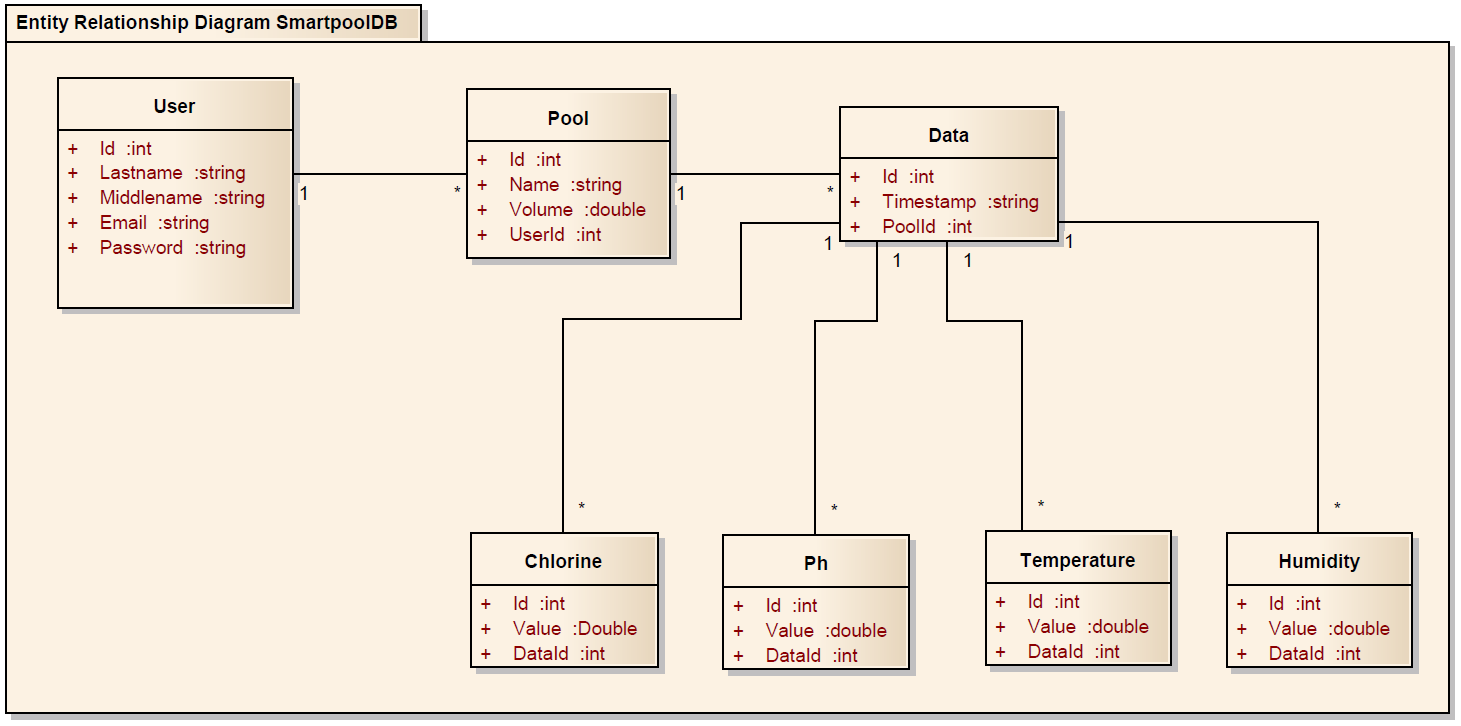
\includegraphics[width=\linewidth]{figs/design/databaseERD_final_uml}
	\caption{Endeligt ER diagram, UML notation}
	\label{fig:databaseERD_final_uml}
\end{figure}

Det endelige database design kan ses på figur~\ref{fig:databaseERD_final_uml}. I modsætning til designet på figur~\ref{fig:databaseERD_firstattempt_uml} er dette design mere simpelt og langt bedre optimeret. Optimeringen ligger til dels i at nogle af entiteterne er samlet til én enkelt, og dels i måden hvorpå data kan hentes ud af databasen. 

\todo{Skriv noget om hvordan man querier på DB her! + noget om hvordan data-pH/chlorine relationen fungerer}

I det nuværende design kan der laves en query på pooldata ved at kalde data getter metoderne i DataAccess klassen. Som det kan ses på figur \ref{fig:getDataClassDiagramPNG} eksponerer DataAccess et interface, IDataAccess der initialiseres i SmartPoolDB klassens constructor.

\begin{figure}[h]
	\centering
	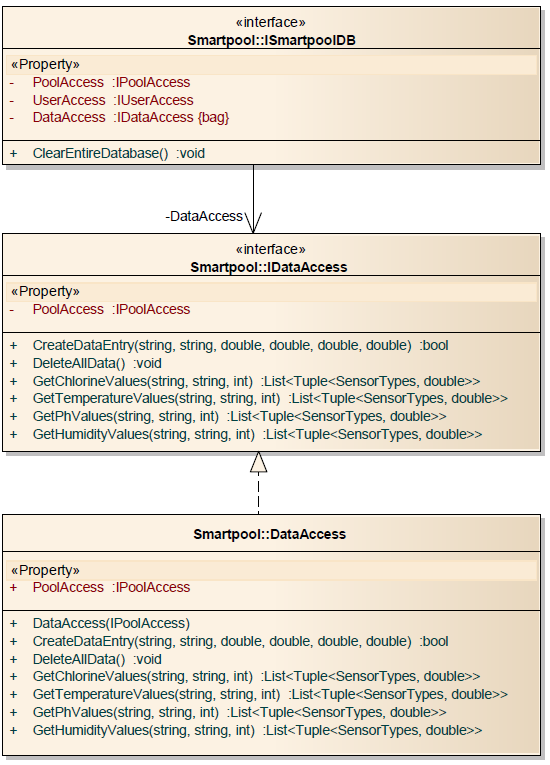
\includegraphics[width=0.7\linewidth]{figs/design/getDataClassDiagramPNG.PNG}
	\caption{Udtag pooldata fra databasen - DataAccess klassediagram}
	\label{fig:getDataClassDiagramPNG}
\end{figure}

Dette designvalg er taget for at simplificere brugen GetData metoder, og for at dependancy inverte forholdet mellem SmartPoolDB og DataAccess. 

\todo{Skriv om DataAcces og IDataAccess}




